\documentclass{article}
\usepackage[utf8]{inputenc}
\usepackage{listings}
\usepackage{xcolor}
\usepackage{graphicx}
\graphicspath{ {../plots/} }

\usepackage{geometry}
 \geometry{
 a4paper,
 total={170mm,257mm},
 left=20mm,
 top=20mm,
}

\definecolor{codegreen}{rgb}{0,0.6,0}
\definecolor{codegray}{rgb}{0.5,0.5,0.5}
\definecolor{codepurple}{rgb}{0.58,0,0.82}
\definecolor{backcolour}{rgb}{0.95,0.95,0.92}

\lstdefinestyle{default_python_style}{
    backgroundcolor=\color{backcolour},   
    commentstyle=\color{codegreen},
    keywordstyle=\color{magenta},
    numberstyle=\tiny\color{codegray},
    stringstyle=\color{codepurple},
    basicstyle=\ttfamily\footnotesize,
    breakatwhitespace=false,         
    breaklines=true,                 
    captionpos=b,                    
    keepspaces=true,                 
    numbers=left,                    
    numbersep=5pt,                  
    showspaces=false,                
    showstringspaces=false,
    showtabs=false,                  
    tabsize=2
}
\lstset{style=default_python_style}

\renewcommand{\lstlistingname}{Kód}
\renewcommand{\figurename}{Obrázek}

\begin{document}
\begin{titlepage}
    \centering
    \vfill
    
\includegraphics[width=0.5\textwidth]{../doc/fit_logo}
    \vfill
    {\Huge{\bfseries{ISS Projekt}}\\
        \Large{Leden 2022}\\
        \vfill
        Augustin Machyňák \\
        xmachy02
    }
    \vfill
\end{titlepage}

\newpage


\section{Úkoly}
Pro řešení projektu byl použit programovací jazyk Python a knihovny
\textit{numpy}, \textit{scipy} a \textit{matplotlib}. 
Kromě materiálů zmíněných v zadání bylo pro realizaci hojně využíváno dokumentace 
již zmíněných knihoven, jelikož se autor s těmito knihovny setkal poprvé v životě.

\begin{lstlisting}[language=Python, caption={Použité knihovny}]
import numpy as np
from scipy.io import wavfile
from scipy import signal
import matplotlib.pyplot as plt
\end{lstlisting}


\subsection{Základy}

\begin{lstlisting}[language=Python, caption={Načtení vstupního signálu}]
def read_file(file_name):
    fs, data = wavfile.read(file_name)
    return fs, data
\end{lstlisting}

\begin{center}
Délka signálu ve vzorcích (\textit{data.size}): 35431 \\
Délka signálu v sekundách (\textit{data.size/fs}): 2.214 [s]\\
Minimální hodnota (\textit{data.min()}): -1996\\
Maximální hodnota (\textit{data.max()}): 3506\\
\end{center}

\begin{figure}[ht]
    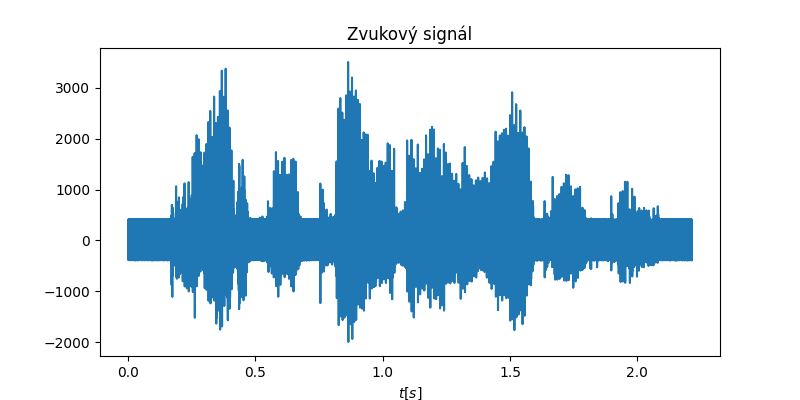
\includegraphics[width=1.0\textwidth]{plot_4_1}
    \caption{Zobrazení vstupního signálu}
\end{figure}

\newpage


\subsection{Předzpracování a rámce}
\begin{lstlisting}[language=Python, caption={Ustřednění signálu a jeho normalizování do dynamického rozsahu}]
def normalize(data):
    new_data = data.copy()
    m = np.mean(new_data, axis=0)
    new_data -= int(m)
    abs_max = np.maximum(np.abs(data.min()), data.max())
    new_data = new_data / abs_max
    return new_data
\end{lstlisting}

\begin{lstlisting}[language=Python, caption={Rozdělení na rámce o velikosti 1024 vzorků s překrytím 512 vzorků}]
def split_512(data):
    new_data = []
    i = 0
    for i in range(0, data.size - 1024, 512):
        new_data.append(data[i:i + 1024])
    i += 512
    if i < data.size:
        new_data.append(data[i:data.size])
    return new_data
\end{lstlisting}

\begin{figure}[ht]
    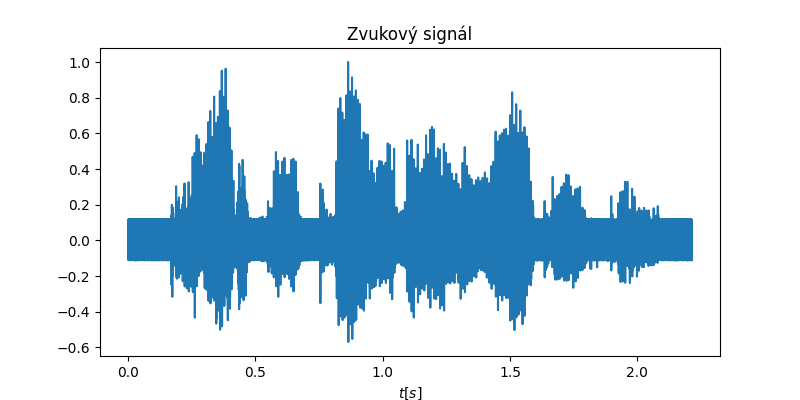
\includegraphics[width=1.0\textwidth]{plot_4_2}
    \caption{Ustředněný a normalizovaný vstupní signál}
\end{figure}

\newpage


\subsection{DFT}
\begin{flushleft}
    Pro implementaci DFT byla využita DFT Matice. DFT je realizována 
    jako násobení této matice s vektorem signálu.

\begin{lstlisting}[language=Python, caption={Implementace DFT}]
def my_dft(data):
    N = data.size
    # dft matrix
    a, b = np.meshgrid(np.arange(0, N), np.arange(0, N))

    # e^ -2*PI*J/N
    w = np.exp(-2 * np.pi * 1J / N)
    matrix = np.power(w, a * b) / np.sqrt(N)

    result = data.dot(matrix)
    return result
\end{lstlisting}

    Bohužel však výsledné hodnoty neodpovídají hodnotám z numpy knihovní implementace FFT.
    Vizuálně výsledek vypadá stejně, ale hodnoty jsou několikanásobně menší (viz následující obrázky).
    Příčina se nepodařila odhalit.

    \begin{figure}[ht]
        \centering
        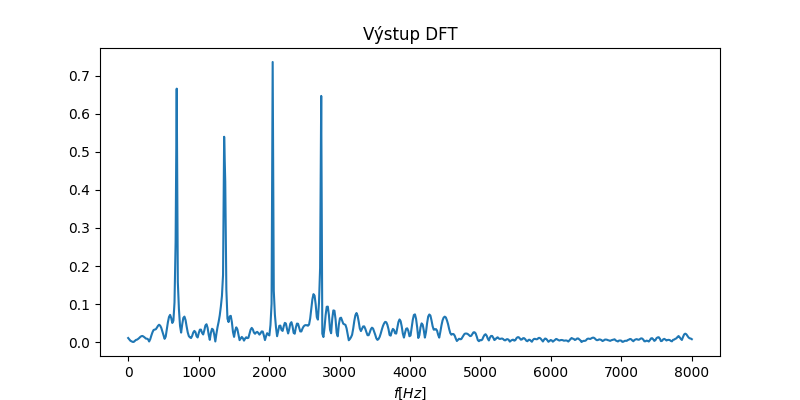
\includegraphics[width=0.85\textwidth]{my_fft}
        \caption{Výsledek vlastní implementace DFT}
    \end{figure}

    \begin{figure}[ht]
        \centering
        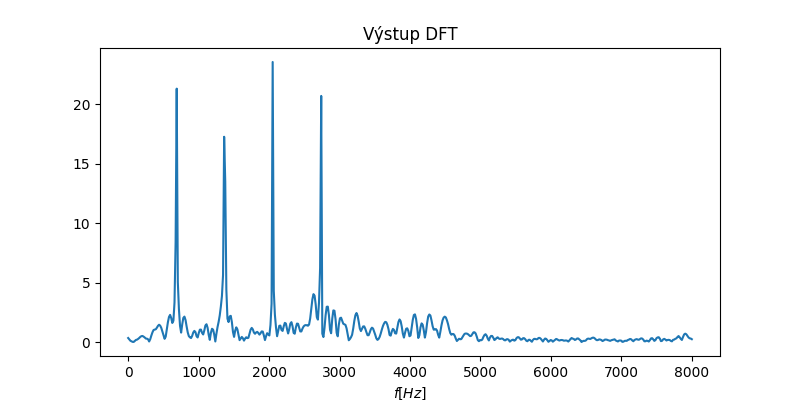
\includegraphics[width=0.85\textwidth]{fft}
        \caption{Výsledek knihovní FFT}
    \end{figure}
\end{flushleft}

\newpage

\subsection{Spektrogram}
\begin{flushleft}

    \begin{figure}[ht]
        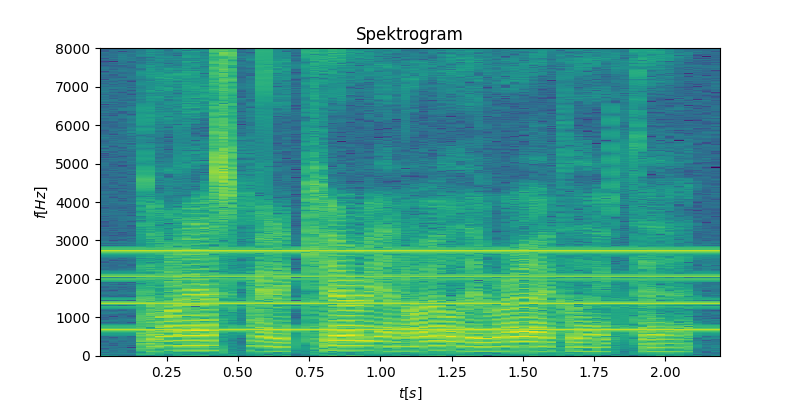
\includegraphics[width=1.0\textwidth]{in_spectro}
        \caption{Spektrogram vstupního signálu}
    \end{figure}

\end{flushleft}


\subsection{Určení rušivých frekvencí} 
\begin{flushleft}
    Pomocí funkce níže (Kód 6) a spektrogramu bylo zjištěno, že rušivé frekvence jsou:
    \begin{center}
    687.5 Hz, 1359.375 Hz, 2046.875 Hz a 2734.375 Hz
    \end{center}

    Tyto frekvence byly následně zprůměrovány pro získání harmonicky vztažených frekvencí následovně: \\
    \[
    f_{avg} = \frac{f_1 + f_2 + f_3 + f_4}{10}
    \]
    \[
    f'_1 = f_{avg} \quad f'_2 = f_{avg} \cdot 2 \quad f'_3 = f_{avg} \cdot 3 \quad f'_4 = f_{avg} \cdot 4
    \]
    \[
        f'_1 = 682.8125 \quad f'_2 = 1365.625 \quad f'_3 = 2048.4375 \quad f'_4 = 2731.25 Hz
    \]

\begin{lstlisting}[language=Python, caption={Funkce pro nalezení 'n' největších hodnot z výsledku DFT/FFT}]
def get_n_max(data, n):
    arr_max = []
    for a in range(0, n):
        arr_max.append([0.0, 0.0])
    for a in range(0, data.size):
        calc_val = np.sqrt(data[a].real**2 + data[a].imag**2)
        for i in range(0, n):
            if calc_val > arr_max[i][0]:
                arr_max[i + 1:n] = arr_max[i:n - 1]
                arr_max[i] = [calc_val, a]
                break
    return arr_max
\end{lstlisting}
\end{flushleft}

\newpage


\subsection{Generování signálu}
\begin{flushleft}

\begin{lstlisting}[language=Python, caption={Funkce pro generování 4 cosinusovek}]
def gen_cosine_waves(fs, data, F):
    AMPL = 500
    t = data.size / fs
    samples = np.arange(t * fs) / fs
    cos = [
        np.int16(np.cos(2 * np.pi * F[0] * samples) * AMPL),
        np.int16(np.cos(2 * np.pi * F[1] * samples) * AMPL),
        np.int16(np.cos(2 * np.pi * F[2] * samples) * AMPL),
        np.int16(np.cos(2 * np.pi * F[3] * samples) * AMPL)
    ]
    return cos

_coss = gen_cosine_waves(_fs, _data, _F)
_4cos = _coss[0] + _coss[1] + _coss[2] + _coss[3]
wavfile.write('audio/4cos.wav', _fs, _4cos)
\end{lstlisting}
    \begin{figure}[ht]
        \centering
        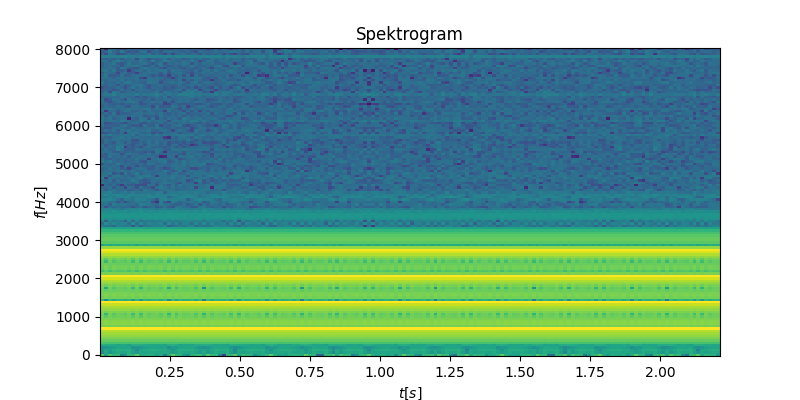
\includegraphics[width=1.0\textwidth]{4cos_spectro}
        \caption{Spektrogram signálu 4 cosinusovek}
    \end{figure}
\end{flushleft}

\newpage


\subsection{Čistící filtr}
\begin{flushleft}
    Byl zvolen filtr podle první alternativy - filtr v z-rovině a byl dodržen postup,
    který byl v zadání navržen.
\begin{lstlisting}[language=Python, caption={Výroba filtru v z-rovině}]
def z_filter_zeros(fs, F):
    omegak = []
    nk = []
    for i in range(0, len(F)):
        omegak.append(2 * np.pi * (F[i] / fs))
        nk.append(np.exp(1J * omegak[i]))
    nk = [*nk, *np.conj(nk)]
    return nk

def z_filter(nk):
    coeff = np.poly(nk)
    return coeff

_filter_zeros = z_filter_zeros(_fs, _F)
_filter_b = z_filter(_filter_zeros)
\end{lstlisting}

    \begin{figure}[ht]
        \centering
        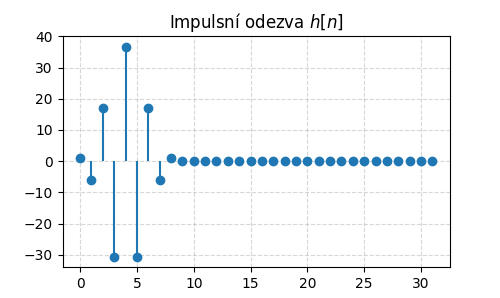
\includegraphics[width=0.6\textwidth]{z_filter_IR}
        \caption{Impulzní odezva filtru v z-rovině}
    \end{figure}

\end{flushleft}

\newpage


\subsection{Nulové body a póly}
\begin{flushleft}
    \begin{figure}[ht]
        \centering
        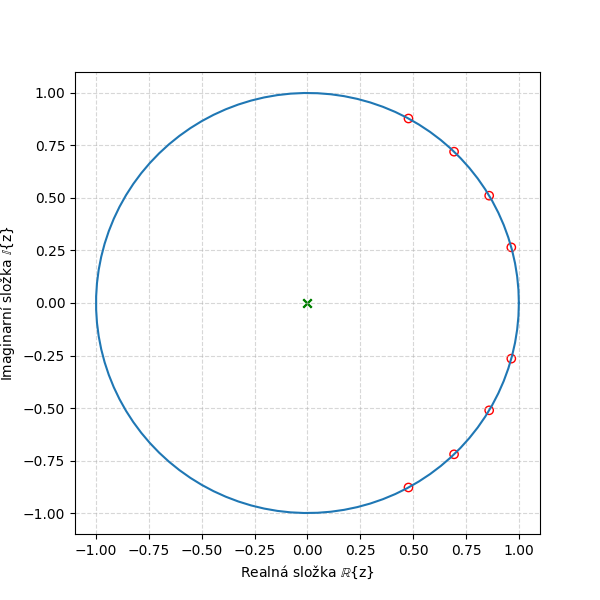
\includegraphics[width=0.5\textwidth]{z_filter_zp}
        \caption{Nulové body a póly filtru (kolečka - nuly, křížky - póly)}
    \end{figure}
\end{flushleft}

\subsection{Frekvenční charakteristika}
\begin{flushleft}
    \begin{figure}[ht]
        \centering
        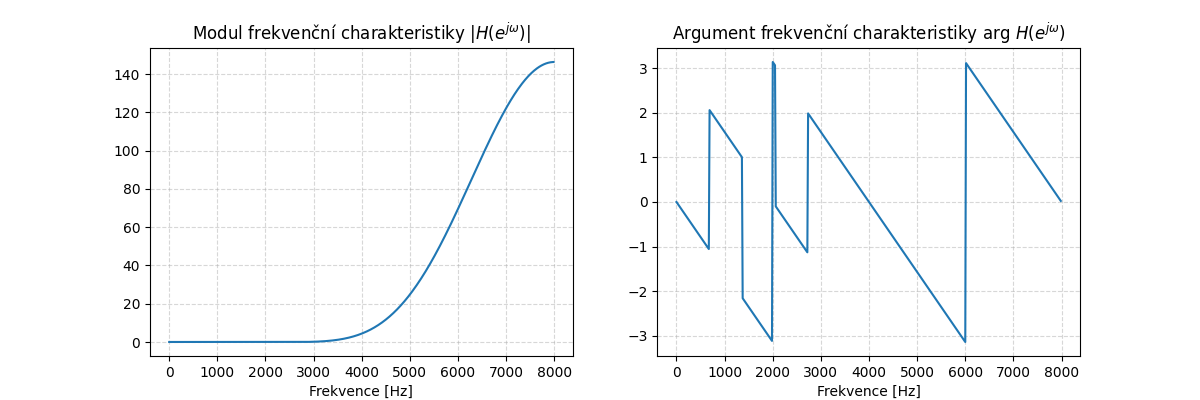
\includegraphics[width=1.0\textwidth]{z_filter_freqz}
        \caption{Frekvenční charakteristika filtru}
    \end{figure}
\end{flushleft}

\subsection{Filtrace}
\begin{flushleft}
    Vstupní signál je vyfiltrován pomocí konvoluce vstupního normalizovaného signálu 
    a koeficientů filtru v z-rovině.
    Následně je signál vynásoben maximální absolutní hodnotou vstupního signálu 
    (pro zpětný přechod z dynamického rozsahu -1 až 1).
\begin{lstlisting}[language=Python, caption={Filtrování}]
_out = np.int16(np.convolve(_data, _filter_b) * _abs_max)
\end{lstlisting}
    Výsledek filtrování je však zklamáním. Výsledný signál je totiž poměrně dost zkreslený.
    Malé zkreslení bylo očekávané, ale zkreslení vypadá, že je až příliš velké. 
    Jsem v domnění, že pravděpodobně došlo někde k chybě při mém postupu, 
    jelikož i frekvenční charakteristika vypadá pochybně.

\end{flushleft}

\begin{lstlisting}[language=Python, caption={}]
\end{lstlisting}

\end{document}